% !TEX program = xelatex
\documentclass[12pt,a4paper,fontset=fandol]{ctexart}
\usepackage{amsmath,amssymb,geometry,booktabs,array,fancyhdr,caption}
\usepackage{pgfplots}
\pgfplotsset{compat=1.18}
\geometry{left=2.2cm,right=2.2cm,top=2.3cm,bottom=2.2cm,headheight=16pt}
\linespread{1.04}
\setlength{\tabcolsep}{4.5pt}
\renewcommand{\arraystretch}{1.15}
\captionsetup{font=small,labelfont=bf,skip=4pt}
\ctexset{
  section={format=\large\bfseries,number=\chinese{section},aftername=、,beforeskip=1.8ex,afterskip=1.0ex},
  subsection={format=\normalsize\bfseries,beforeskip=1.3ex,afterskip=0.7ex}
}
\pagestyle{fancy}\fancyhf{}
\fancyhead[C]{\small 普通物理 I 实验——数据处理}
\fancyfoot[C]{\small\thepage}
\renewcommand{\headrulewidth}{0pt}
\pgfplotsset{labplot/.style={
  width=0.76\linewidth,height=5.0cm,
  axis line style={black},tick style={black},
  tick label style={font=\small},label style={font=\small},
  legend style={font=\small,draw=none,fill=none},
  grid=major,grid style={gray!22},
}}
% calculate.py 自动生成；请修改 data.json 后重新运行。
\newcommand{\PartOneRawRows}{
2.0 & 0.00030 & 3.141$^{*}$ & 2.849 & 2.928 & 2.913 & 2.897 & [2.7588, 3.1324] & 剔除第1次 \\
4.0 & 0.00122 & 3.005 & 3.041 & 3.061 & 3.036 & 3.040 & [3.0033, 3.0699] & 全部保留 \\
8.0 & 0.00487 & 3.048 & 3.040 & 3.038 & 3.043 & 3.041 & [3.0357, 3.0483] & 全部保留 \\
10.0 & 0.00760 & 3.049 & 3.048 & 3.051 & 3.047 & 3.055 & [3.0448, 3.0552] & 全部保留 \\
12.0 & 0.01093 & 3.057 & 3.054 & 3.060 & 3.058 & 3.054 & [3.0523, 3.0609] & 全部保留 \\
24.0 & 0.04323 & 3.073 & 3.072 & 3.073 & 3.071 & 3.065$^{*}$ & [3.0653, 3.0763] & 剔除第5次 \\
32.0 & 0.07598 & 3.099 & 3.094 & 3.098 & 3.099 & 3.095 & [3.0931, 3.1009] & 全部保留 \\}
\newcommand{\PartOneStatRows}{
2.0 & 4 & 2.89675 & 0.03426 & 0.01713 & 3.18 & 0.05447 & 0.05448 & 1.15870 & 0.02179 \\
4.0 & 5 & 3.03660 & 0.02016 & 0.00901 & 2.78 & 0.02506 & 0.02508 & 1.21464 & 0.01003 \\
8.0 & 5 & 3.04200 & 0.00381 & 0.00170 & 2.78 & 0.00473 & 0.00483 & 1.21680 & 0.00193 \\
10.0 & 5 & 3.05000 & 0.00316 & 0.00141 & 2.78 & 0.00393 & 0.00404 & 1.22000 & 0.00162 \\
12.0 & 5 & 3.05660 & 0.00261 & 0.00117 & 2.78 & 0.00324 & 0.00338 & 1.22264 & 0.00135 \\
24.0 & 4 & 3.07225 & 0.00096 & 0.00048 & 3.18 & 0.00152 & 0.00179 & 1.22890 & 0.00072 \\
32.0 & 5 & 3.09700 & 0.00235 & 0.00105 & 2.78 & 0.00292 & 0.00307 & 1.23880 & 0.00123 \\}
\newcommand{\PartTwoRawRows}{
30.000 & 31.000 & 2.746 & 2.747 & 2.789$^{*}$ & 2.757 & 2.753 & [2.7292, 2.7876] & 剔除第3次 \\
33.000 & 34.000 & 2.890 & 2.922 & 2.890 & 2.919 & 2.922 & [2.8805, 2.9367] & 全部保留 \\
36.000 & 37.000 & 3.011 & 3.040 & 3.013 & 3.037 & 3.007 & [2.9958, 3.0474] & 全部保留 \\
39.000 & 40.000 & 3.136 & 3.132 & 3.135 & 3.135 & 3.182$^{*}$ & [3.1089, 3.1791] & 剔除第5次 \\
42.000 & 43.000 & 3.244 & 3.243 & 3.240 & 3.283$^{*}$ & 3.240 & [3.2194, 3.2806] & 剔除第4次 \\}
\newcommand{\PartTwoStatRows}{
31.000 & 4 & 2.75075 & 0.00519 & 0.00259 & 3.18 & 0.00825 & 0.00830 & 1.10030 & 1.21066 & 0.00731 \\
34.000 & 5 & 2.90860 & 0.01702 & 0.00761 & 2.78 & 0.02116 & 0.02119 & 1.16344 & 1.35359 & 0.01972 \\
37.000 & 5 & 3.02160 & 0.01561 & 0.00698 & 2.78 & 0.01941 & 0.01944 & 1.20864 & 1.46081 & 0.01879 \\
40.000 & 4 & 3.13450 & 0.00173 & 0.00087 & 3.18 & 0.00275 & 0.00291 & 1.25380 & 1.57201 & 0.00292 \\
43.000 & 4 & 3.24175 & 0.00206 & 0.00103 & 3.18 & 0.00328 & 0.00341 & 1.29670 & 1.68143 & 0.00354 \\}
\newcommand{\PartOneSlope}{0.7380}
\newcommand{\PartOneSlopeSD}{0.0764}
\newcommand{\PartOneSlopeU}{0.2124}
\newcommand{\PartOneIntercept}{3.04139}
\newcommand{\PartOneInterceptSD}{0.00276}
\newcommand{\PartOneInterceptU}{0.00774}
\newcommand{\PartOneRTwo}{0.9589}
\newcommand{\PartOneR}{0.9792}
\newcommand{\PartOneTZero}{1.21655}
\newcommand{\PartOneTZeroU}{0.00310}
\newcommand{\PartOneTZeroFinal}{(1.2166\pm 0.0031)}
\newcommand{\PartOneTwoTZeroFinal}{(2.4331\pm 0.0062)}
\newcommand{\PartOneG}{9.8429}
\newcommand{\PartOneGU}{0.0517}
\newcommand{\PartOneGFinal}{(9.84\pm 0.05)}
\newcommand{\PartOneGRelU}{0.52\%}
\newcommand{\PartOneGDiff}{+0.049}
\newcommand{\PartOneGRelDiff}{+0.50\%}
\newcommand{\PartTwoSlope}{3.8665}
\newcommand{\PartTwoSlopeSD}{0.1260}
\newcommand{\PartTwoSlopeU}{0.4006}
\newcommand{\PartTwoIntercept}{0.0251}
\newcommand{\PartTwoInterceptSD}{0.0469}
\newcommand{\PartTwoInterceptU}{0.1492}
\newcommand{\PartTwoRTwo}{0.9968}
\newcommand{\PartTwoR}{0.9984}
\newcommand{\PartTwoG}{10.2103}
\newcommand{\PartTwoGU}{1.0580}
\newcommand{\PartTwoGSD}{0.3327}
\newcommand{\PartTwoGFinal}{(10.2\pm 1.1)}
\newcommand{\PartTwoGFinalTwoDigits}{(10.21\pm 1.06)}
\newcommand{\PartTwoGRelU}{10.36\%}
\newcommand{\PartTwoGDiff}{+0.416}
\newcommand{\PartTwoGRelDiff}{+4.25\%}
\newcommand{\PartOnePlotCoords}{(0.001218,3.03660) +- (0,0.02508) (0.004866,3.04200) +- (0,0.00483) (0.007596,3.05000) +- (0,0.00404) (0.010926,3.05660) +- (0,0.00338) (0.043227,3.07225) +- (0,0.00179) (0.075976,3.09700) +- (0,0.00307)}
\newcommand{\PartTwoPlotCoords}{(0.3100,1.21066) +- (0,0.00731) (0.3400,1.35359) +- (0,0.01972) (0.3700,1.46081) +- (0,0.01879) (0.4000,1.57201) +- (0,0.00292) (0.4300,1.68143) +- (0,0.00354)}


\begin{document}
\begin{center}
{\zihao{4}\bfseries 单摆周期测量}\\[6pt]
姓名：姚鉴轩\qquad 学号：2025521024
\end{center}

\section{固定摆长，改变摆角测定重力加速度}
\subsection{实验数据与粗差判别}
测得摆线长度 $L_1=35.900\,\mathrm{cm}$，小球直径 $L_2=1.996\,\mathrm{cm}$，总摆长 $L=L_1+0.5L_2=36.900\,\mathrm{cm}=0.36900\,\mathrm m$。取置信概率 $P=0.95$，米尺仪器误差为 $0.05\,\mathrm{cm}$，游标卡尺仪器误差为 $0.002\,\mathrm{cm}$，则 $U_{L_1}=0.95\times0.05=0.0475\,\mathrm{cm}$，$U_{L_2}=0.95\times0.002=0.0019\,\mathrm{cm}$，总摆长的不确定度为
\[
U_L=\sqrt{U_{L_1}^2+(0.5U_{L_2})^2}
=\sqrt{0.0475^2+0.00095^2}=0.04751\,\mathrm{cm}\approx0.05\,\mathrm{cm},
\]
即 $L=(36.90\pm0.05)\,\mathrm{cm}$。

霍尔传感器位于平衡位置正下方，小球每经过半个周期触发一次。实验中记录 5 次触发，实际经过 $2.5$ 个周期，记测得时间为 $t=2.5T$。不同摆角 $\theta$ 下的测量结果如表 1 所示。
\begin{center}\small
\captionof{table}{改变摆角时的周期测量数据与粗差判别（$t=2.5T$，时间单位：s）}
\begin{tabular}{@{}ccrrrrrrcl@{}}
\toprule
$\theta/^\circ$ & $\sin^2(\theta/2)$ & 1 & 2 & 3 & 4 & 5 & 判别范围/s & 处理\\\midrule
\PartOneRawRows
\bottomrule
\end{tabular}
\end{center}

各组的算术平均值和样本标准差为
\[
\bar t=\frac{1}{n}\sum_{i=1}^n t_i,\qquad
s_t=\sqrt{\frac{\sum_{i=1}^n(t_i-\bar t)^2}{n-1}}.
\]
由肖维涅准则，$n=5$ 时系数取 $c=1.65$，判别范围为 $\bar t\pm1.65s_t$。$\theta=2.0^\circ$ 组第 1 次读数 $3.141\,\mathrm s$ 超出上限 $3.1324\,\mathrm s$，$\theta=24.0^\circ$ 组第 5 次读数 $3.065\,\mathrm s$ 低于下限 $3.0653\,\mathrm s$，均予以剔除并在表 1 中以星号标记；其余各组数据全部保留。

\subsection{周期的不确定度计算}
取置信概率 $P=0.95$，电子计时器仪器误差为 $0.001\,\mathrm s$，平均值标准差、A 类与 B 类不确定度及合成不确定度分别为
\[
s_{\bar t}=\frac{s_t}{\sqrt n},\quad
\Delta_A=t_{0.95}s_{\bar t},\quad
\Delta_B=0.95\times0.001=0.00095\,\mathrm s,\quad
U_t=\sqrt{\Delta_A^2+\Delta_B^2},
\]
其中 $n=5$ 时 $t_{0.95}=2.78$，$n=4$ 时 $t_{0.95}=3.18$。单摆周期 $\bar T=\bar t/2.5$，其不确定度为 $U_T=U_t/2.5$。以 $\theta=8.0^\circ$ 组为例：
\[
\begin{aligned}
\bar t&=\frac{3.048+3.040+3.038+3.043+3.041}{5}=3.04200\,\mathrm s,\qquad s_t=0.00381\,\mathrm s,\\
U_t&=\sqrt{\left(2.78\times\frac{0.003808}{\sqrt5}\right)^2+0.00095^2}=0.00483\,\mathrm s,\qquad
\bar T=(1.2168\pm0.0019)\,\mathrm s.
\end{aligned}
\]
各组统计结果汇总于表 2。
\begin{center}\small
\captionof{table}{改变摆角各组的统计结果（时间量单位均为 s）}
\begin{tabular}{@{}crrrrrrrrr@{}}
\toprule
$\theta/^\circ$ & $n$ & $\bar t$ & $s_t$ & $s_{\bar t}$ & $t_{0.95}$ & $\Delta_A$ & $U_t$ & $\bar T$ & $U_T$\\\midrule
\PartOneStatRows
\bottomrule
\end{tabular}
\end{center}

\subsection{直线拟合与重力加速度计算}
当 $\theta=2.0^\circ$ 时，悬线下端点水平振幅 $x=L_1\sin2.0^\circ\approx1.25\,\mathrm{cm}$，接近霍尔开关导通距离（$1.1\,\mathrm{cm}$），传感器触发不稳定，测得均值明显偏离其余各组。因此拟合时剔除 $\theta=2.0^\circ$ 组，采用 $4.0^\circ\sim32.0^\circ$ 共 6 组数据。由椭圆积分二级近似公式：
\[
T=T_0\left(1+\frac{1}{4}\sin^2\frac{\theta}{2}\right),\qquad
t=2.5T=2.5T_0+\frac{2.5T_0}{4}\sin^2\frac{\theta}{2}.
\]
令 $x=\sin^2(\theta/2)$，$y=\bar t=2.5\bar T$，作最小二乘线性拟合 $y=k_1x+b_1$，拟合图如图 1 所示。
\begin{center}
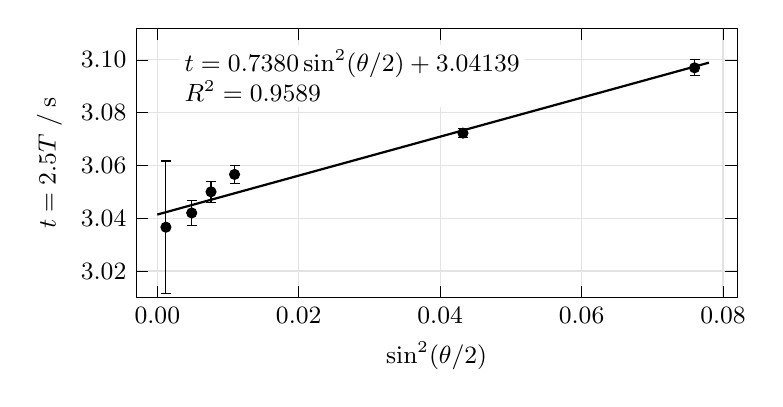
\begin{tikzpicture}
  \begin{axis}[
    labplot,
    xlabel={$\sin^2(\theta/2)$},
    ylabel={$t=2.5T\;/\;\mathrm s$},
    xmin=-0.003, xmax=0.082,
    ymin=3.010, ymax=3.112,
    xtick={0,0.02,0.04,0.06,0.08},
    ytick={3.02,3.04,3.06,3.08,3.10},
    scaled x ticks=false,
    xticklabel style={/pgf/number format/fixed,/pgf/number format/fixed zerofill,/pgf/number format/precision=2},
    yticklabel style={/pgf/number format/fixed,/pgf/number format/fixed zerofill,/pgf/number format/precision=2},
  ]
    \addplot[
      only marks, mark=*, mark size=1.8pt, black,
      error bars/.cd, y dir=both, y explicit
    ] coordinates {\PartOnePlotCoords};
    \addplot[black, thick, domain=0:0.078, samples=2] {\PartOneSlope*x + \PartOneIntercept};
    \node[anchor=north west, font=\small, align=left, fill=white, inner sep=2pt] at (axis cs:0.003,3.106)
      {$t=\PartOneSlope\sin^2(\theta/2)+\PartOneIntercept$\\$R^2=\PartOneRTwo$};
  \end{axis}
\end{tikzpicture}
\captionof{figure}{$t=2.5T$ 与 $\sin^2(\theta/2)$ 的线性拟合关系（误差棒表示 $P=0.95$ 下的不确定度 $U_t$）}
\end{center}

线性回归求得斜率 $k_1=\PartOneSlope\,\mathrm s$（标准差 $s_{k_1}=\PartOneSlopeSD\,\mathrm s$），截距 $b_1=2.5T_0=\PartOneIntercept\,\mathrm s$（标准差 $s_{b_1}=\PartOneInterceptSD\,\mathrm s$），决定系数 $R^2=\PartOneRTwo$（相关系数 $r=\PartOneR$）。拟合点个数 $m=6$，自由度 $\nu=m-2=4$，取 $t_{0.95}=2.78$，截距不确定度及外推零摆角周期 $T_0$ 为
\[
\begin{aligned}
U_{b_1}&=\sqrt{(t_{0.95}s_{b_1})^2+\Delta_B^2}
=\sqrt{(2.78\times0.002762)^2+0.00095^2}=\PartOneInterceptU\,\mathrm s,\\
T_0&=\frac{b_1}{2.5}=\PartOneTZero\,\mathrm s,\qquad
U_{T_0}=\frac{U_{b_1}}{2.5}=\PartOneTZeroU\,\mathrm s,
\end{aligned}
\]
即 $T_0=\PartOneTZeroFinal\,\mathrm s$（对应二倍周期 $2T_0=\PartOneTwoTZeroFinal\,\mathrm s$）。由 $g_1=4\pi^2L/T_0^2$ 计算重力加速度及其不确定度：
\[
\begin{aligned}
g_1&=\frac{4\pi^2L}{T_0^2}
=\frac{4\pi^2\times0.36900}{1.216555^2}=\PartOneG\,\mathrm{m\,s^{-2}},\\
U_{g_1}&=g_1\sqrt{\left(\frac{U_L}{L}\right)^2+\left(\frac{2U_{T_0}}{T_0}\right)^2}
=9.8429\sqrt{\left(\frac{0.04751}{36.900}\right)^2+\left(\frac{2\times0.003095}{1.216555}\right)^2}
=\PartOneGU\,\mathrm{m\,s^{-2}}.
\end{aligned}
\]
因此，固定摆长法测得 $g_1=\PartOneGFinal\,\mathrm{m\,s^{-2}}$，相对不确定度为 \PartOneGRelU。与参考值 $g_{\mathrm{ref}}=9.794\,\mathrm{m\,s^{-2}}$ 相比，绝对偏差为 $\PartOneGDiff\,\mathrm{m\,s^{-2}}$，相对偏差为 \PartOneGRelDiff。

\section{改变摆长测定重力加速度}
\subsection{实验数据与粗差判别}
保持小摆角条件（$\theta<3^\circ$），改变摆线长度 $L_1$，测量 5 组不同总摆长 $L=L_1+0.5L_2$ 下经过 $2.5$ 个周期的时间 $t=2.5T$，原始数据与肖维涅粗差判别（$n=5$，$c=1.65$）结果如表 3 所示。
\begin{center}\small
\captionof{table}{改变摆长时的周期测量数据与粗差判别（$t=2.5T$，时间单位：s）}
\begin{tabular}{@{}ccrrrrrrcl@{}}
\toprule
$L_1/\mathrm{cm}$ & $L/\mathrm{cm}$ & 1 & 2 & 3 & 4 & 5 & 判别范围/s & 处理\\\midrule
\PartTwoRawRows
\bottomrule
\end{tabular}
\end{center}
$L=31.000\,\mathrm{cm}$ 组第 3 次读数 $2.789\,\mathrm s$、$L=40.000\,\mathrm{cm}$ 组第 5 次读数 $3.182\,\mathrm s$、$L=43.000\,\mathrm{cm}$ 组第 4 次读数 $3.283\,\mathrm s$ 超出各自判别上限，予以剔除并在表 3 中以星号标记，该三组各保留 4 次数据；$L=34.000\,\mathrm{cm}$ 与 $37.000\,\mathrm{cm}$ 两组全部保留。

\subsection{周期平方的不确定度计算}
由 $\bar T=\bar t/2.5$、$U_T=U_t/2.5$，计算周期平方 $T^2=\bar T^2$ 及其不确定度 $U_{T^2}=2\bar T U_T=\frac{4}{5}\bar T U_t$。以 $L=31.000\,\mathrm{cm}$ 组为例，剔除第 3 次读数后（$n=4$，$t_{0.95}=3.18$）：
\[
\begin{aligned}
\bar t&=\frac{2.746+2.747+2.757+2.753}{4}=2.75075\,\mathrm s,\qquad s_t=0.00519\,\mathrm s,\\
U_t&=\sqrt{\left(3.18\times\frac{0.005188}{\sqrt4}\right)^2+0.00095^2}=0.00830\,\mathrm s,\qquad
\bar T=1.10030\,\mathrm s,\\
T^2&=1.10030^2=1.21066\,\mathrm{s^2},\qquad
U_{T^2}=2\times1.10030\times\frac{0.008304}{2.5}=0.00731\,\mathrm{s^2}.
\end{aligned}
\]
其余各组计算结果汇总于表 4。
\begin{center}\small
\captionof{table}{改变摆长各组的统计结果与周期平方（时间单位：s，$T^2$ 单位：$\mathrm{s^2}$）}
\begin{tabular}{@{}crrrrrrrrrr@{}}
\toprule
$L/\mathrm{cm}$ & $n$ & $\bar t$ & $s_t$ & $s_{\bar t}$ & $t_{0.95}$ & $\Delta_A$ & $U_t$ & $\bar T$ & $T^2$ & $U_{T^2}$\\\midrule
\PartTwoStatRows
\bottomrule
\end{tabular}
\end{center}

\subsection{直线拟合与重力加速度计算}
由小摆角下单摆周期公式 $T^2=(4\pi^2/g)L$，以总摆长 $L$（单位：$\mathrm m$）为横坐标、$T^2$（单位：$\mathrm{s^2}$）为纵坐标作最小二乘线性拟合 $T^2=k_2L+a_2$，拟合图如图 2 所示。
\begin{center}
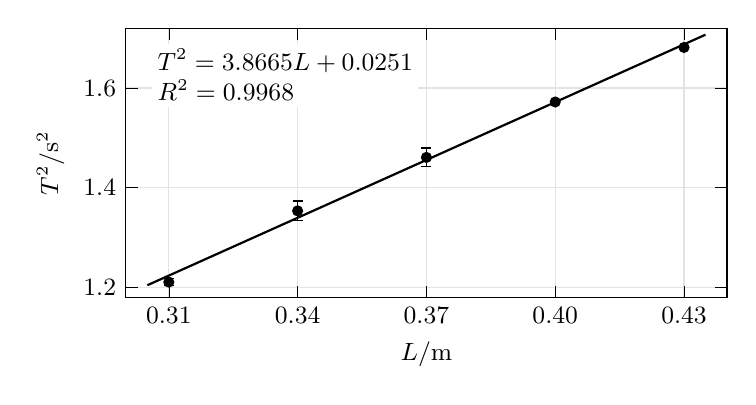
\begin{tikzpicture}
  \begin{axis}[
    labplot,
    xlabel={$L/\mathrm m$},
    ylabel={$T^2/\mathrm{s^2}$},
    xmin=0.300, xmax=0.440,
    ymin=1.18, ymax=1.72,
    xtick={0.31,0.34,0.37,0.40,0.43},
    xticklabel style={/pgf/number format/fixed,/pgf/number format/fixed zerofill,/pgf/number format/precision=2},
    yticklabel style={/pgf/number format/fixed,/pgf/number format/fixed zerofill,/pgf/number format/precision=1},
  ]
    \addplot[
      only marks, mark=*, mark size=1.8pt, black,
      error bars/.cd, y dir=both, y explicit
    ] coordinates {\PartTwoPlotCoords};
    \addplot[black, thick, domain=0.305:0.435, samples=2] {\PartTwoSlope*x + \PartTwoIntercept};
    \node[anchor=north west, font=\small, align=left, fill=white, inner sep=2pt] at (axis cs:0.306,1.69)
      {$T^2=\PartTwoSlope L+\PartTwoIntercept$\\$R^2=\PartTwoRTwo$};
  \end{axis}
\end{tikzpicture}
\captionof{figure}{$T^2$ 与摆长 $L$ 的线性拟合关系（误差棒表示 $P=0.95$ 下的不确定度 $U_{T^2}$）}
\end{center}

线性回归求得斜率 $k_2=\PartTwoSlope\,\mathrm{s^2\,m^{-1}}$（斜率标准差 $s_{k_2}=\PartTwoSlopeSD\,\mathrm{s^2\,m^{-1}}$），截距 $a_2=\PartTwoIntercept\,\mathrm{s^2}$（截距标准差 $s_{a_2}=\PartTwoInterceptSD\,\mathrm{s^2}$），决定系数 $R^2=\PartTwoRTwo$（相关系数 $r=\PartTwoR$），说明 $T^2$ 与 $L$ 呈良好的正比线性关系。拟合点个数 $m=5$，自由度 $\nu=m-2=3$，取 $t_{0.95}=3.18$，斜率的不确定度及重力加速度分别为
\[
U_{k_2}=t_{0.95}s_{k_2}=3.18\times0.12599=\PartTwoSlopeU\,\mathrm{s^2\,m^{-1}},
\]
\[
g_2=\frac{4\pi^2}{k_2}=\frac{4\pi^2}{3.86654}=\PartTwoG\,\mathrm{m\,s^{-2}},\qquad
U_{g_2}=g_2\frac{U_{k_2}}{k_2}
=10.2103\times\frac{0.40064}{3.86654}=\PartTwoGU\,\mathrm{m\,s^{-2}}.
\]
因此，改变摆长法测得 $g_2=\PartTwoGFinal\,\mathrm{m\,s^{-2}}$，相对不确定度为 \PartTwoGRelU。与参考值 $g_{\mathrm{ref}}=9.794\,\mathrm{m\,s^{-2}}$ 相比，绝对偏差为 $\PartTwoGDiff\,\mathrm{m\,s^{-2}}$，相对偏差为 \PartTwoGRelDiff。

\section{实验结论}
1. 固定摆长 $L=(36.90\pm0.05)\,\mathrm{cm}$，在 $4.0^\circ\sim32.0^\circ$ 范围内测得周期随摆角增大而增大，$t=2.5T$ 与 $\sin^2(\theta/2)$ 呈线性关系（$R^2=\PartOneRTwo$）。外推得零摆角周期 $T_0=\PartOneTZeroFinal\,\mathrm s$，求得重力加速度为
\[
\boxed{g_1=\PartOneGFinal\,\mathrm{m\,s^{-2}},}
\]
相对不确定度为 \PartOneGRelU（$P=0.95$），与参考值 $9.794\,\mathrm{m\,s^{-2}}$ 的相对偏差为 \PartOneGRelDiff。

2. 小摆角下改变摆长（$L=31.000\sim43.000\,\mathrm{cm}$），测得 $T^2$ 与 $L$ 呈良好的线性正比关系（$R^2=\PartTwoRTwo$），由拟合斜率 $k_2=(\PartTwoSlope\pm\PartTwoSlopeU)\,\mathrm{s^2\,m^{-1}}$ 求得重力加速度为
\[
\boxed{g_2=\PartTwoGFinal\,\mathrm{m\,s^{-2}},}
\]
相对不确定度为 \PartTwoGRelU（$P=0.95$），与参考值的相对偏差为 \PartTwoGRelDiff。两种方法所得结果均在各自不确定度范围内与参考值一致，其中固定摆长外推法的随机离散更小、精度更高。

\section{误差分析}
1. 霍尔传感器触发位置与小摆角限制：集成霍尔开关的导通距离约为 $1.1\,\mathrm{cm}$。当摆角过小（如第一部分 $\theta=2.0^\circ$，水平位移仅约 $1.25\,\mathrm{cm}$）时，磁钢在极限位置附近刚脱离导通区即返回，易发生提前触发或多次抖动触发，使测得的周期显著偏小（均值仅 $2.897\,\mathrm s$）且离散度增大。此外，若改变摆长后霍尔开关高度未及时调节至小球正下方约 $1.0\,\mathrm{cm}$ 处，或标尺拧紧时发生微小偏转使传感器偏离最低点，触发时间间隔将不再对称，引起系统偏差。实验中每次调节摆长后均应重新校准传感器高度与对中位置，摆角不宜小于 $4^\circ$。

2. 手动释放小球与圆锥摆效应：人工释放小球时，若悬线未完全拉直或手部附有初速度，摆线张力突变会引起小球轻微上下跳动并改变有效摆幅；若释放方向偏离支架所在铅垂面，单摆将混入椭圆（圆锥摆）运动。圆锥摆周期 $T'=2\pi\sqrt{L\cos\alpha/g}$ 小于平面单摆周期，会使测得的 $T$ 偏小，从而使算出的 $g$ 偏大（第二部分 $g_2=10.2\,\mathrm{m\,s^{-2}}$ 略偏大即与此有关）。可通过观察每次经过平衡位置时指示灯是否稳定闪烁来检验平面性，或改用电磁铁/继电器控制小球无初速释放。

3. 摆长测量与横轴跨度限制：调节旋钮改变摆长时，悬线张紧程度、末端基准线对齐视差以及摆动过程中悬点夹持处的微小滑动，都会使实际有效摆长与静态米尺读数产生偏差。在第二部分中，总摆长仅跨越 $0.31\,\mathrm m\sim0.43\,\mathrm m$（跨度 $\Delta L=0.12\,\mathrm m$），较窄的横轴跨度放大了各组时间和摆长起伏对拟合斜率 $k_2$ 的影响（自由度 $\nu=3$，使 $U_{g_2}$ 达 $1.1\,\mathrm{m\,s^{-2}}$）。在器材高度允许范围内，应扩大摆长测量跨度并增加摆长取点组数，以减小斜率的回归不确定度。

\section{思考题}
\noindent\textbf{1. 传统秒表计时测量 $30T$ 而不是直接测 $T$ 是因为什么原因？本实验中有必要测 $30T$ 吗？}

\noindent\textbf{答：}（1）传统秒表由人工观察小球经过平衡位置并手动按表，启动和停止时均存在人体反应时间延迟及位置判断视差，单次启停计时误差达 $0.1\sim0.2\,\mathrm s$。若直接测量 $1$ 个周期（约 $1.2\,\mathrm s$），计时相对误差高达 $10\%$ 以上。若连续测量 $30$ 个周期的总时间 $t=30T$，人工启停误差仅在首尾发生一次，折算至单周期 $T=t/30$ 时，随机启停误差被缩小为原来的 $1/30$（约 $0.003\sim0.007\,\mathrm s$），从而大幅降低单周期的测量不确定度。

（2）本实验中没有必要测 $30T$。一方面，本实验采用集成霍尔开关与 HTM 电子计时器自动触发计时，仪器误差仅为 $0.001\,\mathrm s$，消除了人工反应时间误差，测量 $2.5T$（或 $2T$）时单周期仪器不确定度已小至 $4\times10^{-4}\,\mathrm s$ 量级；另一方面，单摆受空气阻力和悬点阻尼作用，摆角会随摆动次数增加而逐渐衰减。若连续测量 $30T$，首尾摆角变化显著，既无法在第一部分准确测定特定摆角 $\theta$ 对应的周期，又容易因振幅衰减或摆面微偏导致磁钢偏离霍尔开关感应距离而漏计信号。

\medskip
\noindent\textbf{2. 测量 $L$ 不远大于小球半径时周期与上述周期公式的偏差，对比周期 $T$ 的实验记录与公式（4）理论预测之间的偏差，并找出该偏差与 $d/L$ 的关系。}

\noindent\textbf{答：}当摆长 $L$ 不远大于小球半径 $r=d/2$ 时，小球不能再近似为质点，必须作为绕悬点定轴转动的刚体（物理摆）处理。忽略悬线质量，质量为 $m$、直径为 $d=2r$ 的均匀实心球绕球心轴的转动惯量为 $I_C=\frac{2}{5}mr^2=\frac{1}{10}md^2$。由平行轴定理，小球绕悬点的总转动惯量为
\[
I=I_C+mL^2=mL^2\left[1+\frac{2}{5}\left(\frac{r}{L}\right)^2\right]
=mL^2\left[1+\frac{1}{10}\left(\frac{d}{L}\right)^2\right].
\]
在小摆角（$\theta<3^\circ$）条件下，由物理摆周期公式可得实际周期 $T$ 与理想质点单摆公式（4）预测值 $T_0=2\pi\sqrt{L/g}$ 的关系及周期相对偏差为
\[
T=2\pi\sqrt{\frac{I}{mgL}}
=T_0\sqrt{1+\frac{1}{10}\left(\frac{d}{L}\right)^2},\qquad
\frac{T-T_0}{T_0}=\sqrt{1+\frac{1}{10}\left(\frac{d}{L}\right)^2}-1
\approx\frac{1}{20}\left(\frac{d}{L}\right)^2.
\]
由此可知，当 $L$ 较小时，实际周期 $T$ 系统性地大于公式（4）的预测值 $T_0$，且相对偏差近似与 $(d/L)^2$ 成正比。以本实验小球直径 $d\approx2.00\,\mathrm{cm}$ 为例：当 $L=50\,\mathrm{cm}$、$30\,\mathrm{cm}$ 时，$d/L$ 分别为 $0.040$、$0.067$，刚体转动惯量引起的周期相对偏差仅为 $0.008\%$ 和 $0.022\%$，质点近似完全适用；当摆长缩短至 $L=10\,\mathrm{cm}$、$5\,\mathrm{cm}$ 时，$d/L$ 增大至 $0.20$ 和 $0.40$，周期相对偏差分别增大至约 $0.20\%$ 和 $0.80\%$。实验上对 $L=5\,\mathrm{cm}$、$10\,\mathrm{cm}$ 摆长采用秒表连续测量 $20$ 个周期（重复 $3\sim5$ 次）求得 $T_{\mathrm{exp}}$，以 $(T_{\mathrm{exp}}-T_0)/T_0$ 对 $(d/L)^2$ 作图即可验证上述正比关系。
\end{document}
